\documentclass[rusmathsym, eqnumwithinsec, amspack, hyperref]{bomgost}

\DeclareTextSymbol{\CYRA}\UnicodeEncodingName{"0410}        % А
\DeclareTextSymbol{\cyra}\UnicodeEncodingName{"0430}        % а
\DeclareTextSymbol{\CYRB}\UnicodeEncodingName{"0411}        % Б
\DeclareTextSymbol{\cyrb}\UnicodeEncodingName{"0431}        % б
\DeclareTextSymbol{\CYRV}\UnicodeEncodingName{"0412}        % В 
\DeclareTextSymbol{\cyrv}\UnicodeEncodingName{"0432}        % в
\DeclareTextSymbol{\CYRG}\UnicodeEncodingName{"0413}        % Г
\DeclareTextSymbol{\cyrg}\UnicodeEncodingName{"0433}        % г
\DeclareTextSymbol{\CYRD}\UnicodeEncodingName{"0414}        % Д
\DeclareTextSymbol{\cyrd}\UnicodeEncodingName{"0434}        % д
\DeclareTextSymbol{\CYRE}\UnicodeEncodingName{"0415}        % Е 
\DeclareTextSymbol{\cyre}\UnicodeEncodingName{"0435}        % е
\DeclareTextSymbol{\CYRZH}\UnicodeEncodingName{"0416}       % Ж 
\DeclareTextSymbol{\cyrzh}\UnicodeEncodingName{"0436}       % ж
\DeclareTextSymbol{\CYRZ}\UnicodeEncodingName{"0417}        % З
\DeclareTextSymbol{\cyrz}\UnicodeEncodingName{"0437}        % з
\DeclareTextSymbol{\CYRI}\UnicodeEncodingName{"0418}        % И
\DeclareTextSymbol{\cyri}\UnicodeEncodingName{"0438}        % и
\DeclareTextSymbol{\CYRISHRT}\UnicodeEncodingName{"0419}    % Й
\DeclareTextSymbol{\cyrishrt}\UnicodeEncodingName{"0439}    % й
\DeclareTextSymbol{\CYRK}\UnicodeEncodingName{"041A}        % К
\DeclareTextSymbol{\cyrk}\UnicodeEncodingName{"043A}        % к
\DeclareTextSymbol{\CYRL}\UnicodeEncodingName{"041B}        % Л
\DeclareTextSymbol{\cyrl}\UnicodeEncodingName{"043B}        % л 
\DeclareTextSymbol{\CYRM}\UnicodeEncodingName{"041C}        % М
\DeclareTextSymbol{\cyrm}\UnicodeEncodingName{"043C}        % м
\DeclareTextSymbol{\CYRN}\UnicodeEncodingName{"041D}        % Н
\DeclareTextSymbol{\cyrn}\UnicodeEncodingName{"043D}        % н
\DeclareTextSymbol{\CYRO}\UnicodeEncodingName{"041E}        % О
\DeclareTextSymbol{\cyro}\UnicodeEncodingName{"043E}        % о
\DeclareTextSymbol{\CYRP}\UnicodeEncodingName{"041F}        % П
\DeclareTextSymbol{\cyrp}\UnicodeEncodingName{"043F}        % п
\DeclareTextSymbol{\CYRR}\UnicodeEncodingName{"0420}        % Р
\DeclareTextSymbol{\cyrr}\UnicodeEncodingName{"0440}        % р
\DeclareTextSymbol{\CYRS}\UnicodeEncodingName{"0421}        % С
\DeclareTextSymbol{\cyrs}\UnicodeEncodingName{"0441}        % с
\DeclareTextSymbol{\CYRT}\UnicodeEncodingName{"0422}        % Т
\DeclareTextSymbol{\cyrt}\UnicodeEncodingName{"0442}        % т
\DeclareTextSymbol{\CYRU}\UnicodeEncodingName{"0423}        % У
\DeclareTextSymbol{\cyru}\UnicodeEncodingName{"0443}        % у
\DeclareTextSymbol{\CYRF}\UnicodeEncodingName{"0424}        % Ф
\DeclareTextSymbol{\cyrf}\UnicodeEncodingName{"0444}        % ф
\DeclareTextSymbol{\CYRH}\UnicodeEncodingName{"0425}        % Х
\DeclareTextSymbol{\cyrh}\UnicodeEncodingName{"0445}        % х
\DeclareTextSymbol{\CYRC}\UnicodeEncodingName{"0426}        % Ц
\DeclareTextSymbol{\cyrc}\UnicodeEncodingName{"0446}        % ц
\DeclareTextSymbol{\CYRCH}\UnicodeEncodingName{"0427}       % Ч
\DeclareTextSymbol{\cyrch}\UnicodeEncodingName{"0447}       % ч
\DeclareTextSymbol{\CYRSH}\UnicodeEncodingName{"0428}       % Ш
\DeclareTextSymbol{\cyrsh}\UnicodeEncodingName{"0448}       % ш
\DeclareTextSymbol{\CYRSHCH}\UnicodeEncodingName{"0429}     % Щ
\DeclareTextSymbol{\cyrshch}\UnicodeEncodingName{"0449}     % щ
\DeclareTextSymbol{\CYRHRDSN}\UnicodeEncodingName{"042A}    % Ъ
\DeclareTextSymbol{\cyrhrdsn}\UnicodeEncodingName{"044A}    % ъ
\DeclareTextSymbol{\CYRERY}\UnicodeEncodingName{"042B}      % Ы
\DeclareTextSymbol{\cyrery}\UnicodeEncodingName{"044B}      % ы
\DeclareTextSymbol{\CYRSFTSN}\UnicodeEncodingName{"042C}    % Ь
\DeclareTextSymbol{\cyrsftsn}\UnicodeEncodingName{"044C}    % ь
\DeclareTextSymbol{\CYREREV}\UnicodeEncodingName{"042D}     % Э
\DeclareTextSymbol{\cyrerev}\UnicodeEncodingName{"044D}     % э
\DeclareTextSymbol{\CYRYU}\UnicodeEncodingName{"042E}       % Ю
\DeclareTextSymbol{\cyryu}\UnicodeEncodingName{"044E}       % ю
\DeclareTextSymbol{\CYRYA}\UnicodeEncodingName{"042F}       % Я
\DeclareTextSymbol{\cyrya}\UnicodeEncodingName{"044F}       % я

% Закомментируйте это, если hyperref не нужен. 
% Изменение уровня \subparagraph (приложения) в закладках pdf документа. 
% Это нужно для сохранения правильной иерархии закладок в pdf документе.
\makeatletter%
\renewcommand{\toclevel@subparagraph}{2}%
\makeatother% 

% Для вставки программного кода.
\usepackage{listings}

% "Умная" запятая: \(0,2\) - число, \(0, 2\) - перечисление.
\usepackage{icomma}
\usepackage{float}
\usepackage{pgfplots}
\usepackage{pgfplotstable}
\usepackage{longtable}
\usepackage{cleveref}


\pgfplotsset{compat=newest}

\pgfplotstableset{set thousands separator={}, precision=3, use comma, col sep=comma, header=true,
every head row/.style={before row=\hline, after row=\hline},
every even row/.style={after row=\hline},
every odd row/.style={after row=\hline},
every column/.style={column type/.add={|}{}},
every last column/.style={column type/.add={}{|}},
columns/text/.style={string type},
}

\author{}
\title{Пример на основе класса документа \texttt{bomgost.cls}}
\date{\today}


\begin{document}

\maketitle
\thispagestyle{empty}
\newpage

\begin{abstract}
% Для добавления общего числа приложений нужно добавить команду \printtotapp[.]
% Во всех командах существует необязательный аргумент, который добавляется в конец команды. По умолчанию это запятая. Это нужно для случаев, когда каких-то элементов в работе нет т. е. их счётчики равны 0. В этом случае команда ничего не выведет. Так как порядок команд может быть любым и необходимо, чтобы после последней команды была точка, а между командами запятая, поэтому добавлен необязательный аргумент.
Выпускная квалификационная работа содержит \printtotpage \printtotfig \printtottab \printtotref[.] В~некоторых случаях количество приложений не указывается. 

% Для количества приложений команда аналогична: \total{totappendix}~приложений.

КЛЮЧЕВОЕ СЛОВО~1, КЛЮЧЕВОЕ СЛОВО~2, КЛЮЧЕВОЕ СЛОВО~3 и т. д.

Краткое описание работы.
\end{abstract}


\tableofcontents


\section*{ОБОЗНАЧЕНИЯ И СОКРАЩЕНИЯ}
ОДУ - обыкновенные дифференциальные уравнения.

СЛАУ - система линейных алгебраических уравнений.


\section*{ВВЕДЕНИЕ}
Текст введения.


\mainpart


\section{ТЕОРЕТИЧЕСКАЯ ЧАСТЬ}
\subsection{Первый подраздел}
\subsubsection{Максимальный уровень}
Здесь какой - то текст. Квадратное уравнение.

\begin{equation}
f(x) = x^2 + x-2.
\end{equation}

\subsubsection{Рисунок}
График представлен на рисунке ниже.
% Важно добавлять каждый рисунок в окружение gostfigure, чтобы был правильный подсчёт общего числа рисунков.
\begin{gostfigure}
\begin{figure}[H]
\centering
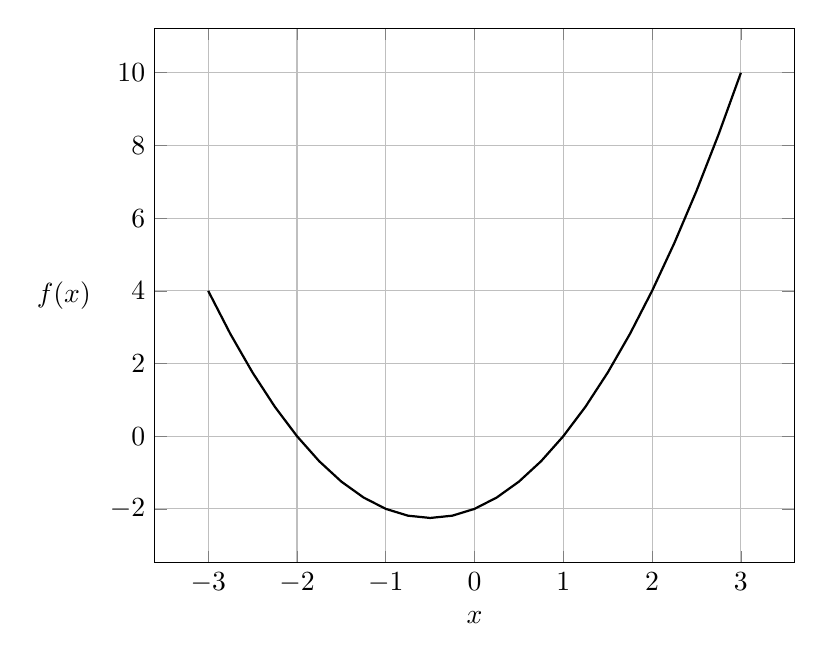
\begin{tikzpicture}
  \begin{axis}[domain=-3:3, width = 0.8 \textwidth, grid = both, ylabel style={rotate=-90}, xlabel = \(x\), ylabel = \(f(x)\)]
  \addplot[mark=none, thick]{x*x + x - 2};
  \end{axis}
\end{tikzpicture}
\caption{График \(f(x)\).}
\end{figure}
\end{gostfigure}

Корни квадратного уравнения представлены в~таблице~\ref{tab:roots}.
% Аналогично с таблицами.
\begin{gosttable}
\begin{table}[H]
\centering
\caption{Корни квадратного уравнения.}
\label{tab:roots}
\begin{tabular}{|c|c|}
\hline 
Первый корень &  Второй корень \\ 
\hline 
1 & -2  \\ 
\hline 
\end{tabular}
\end{table}
\end{gosttable}

\subsection{Таблица из файла}

Пример таблицы из файла, которую просто обновлять.

\pgfplotstableread{data/sample.csv}{\loadedtable}

\begin{gosttable}
    \begin{table}[H]
        \centering
        \caption{Табличные данные}
        \pgfplotstabletypeset[columns={id,num}]{\loadedtable}
    \end{table}
\end{gosttable}

Другие столбцы.

\begin{gosttable}
  \begin{table}[H]
      \centering
      \caption{Табличные данные}
      \pgfplotstabletypeset[columns={id,text}]{\loadedtable}
  \end{table}
\end{gosttable}

\subsubsection{Таблица с разрывом страницы}
\pgfplotstableread{data/big.csv}{\loadedtable}
\begin{gosttable}
  \pgfplotstabletypeset[font=\small
  ,begin table = \begin{longtable}
  ,end table = \end{longtable}
  ,every head row/.append style={before  row={%
  \caption{Таблица с разрывом}
  \label{tab:long_table}\\
  \hline
  \endfirsthead
  \caption*{Продолжение таблицы~\cref{tab:long_table}}\\
  \hline 
  col 1 & col 2 & col 3\\
  \hline
  \endhead
  }
  }
  ,every first row/.append style={before row ={
    col 1 & col 2 & col 3\\
  \hline
  }
  }
  , columns={id,num,text}
  ]{\loadedtable}
\end{gosttable}


\section{ПРАКТИЧЕСКАЯ ЧАСТЬ}
\subsection{Дифференцирование}
\subsubsection{Дифференцирование квадратного уравнения}
\begin{equation}
\dfrac{d f(x)}{d x} = 2 x + 1.
\end{equation}

\section*{ЗАКЛЮЧЕНИЕ}
Интересная стать~\cite{Cybenko}, связанная с~нейронными сетями.

% Список литературы.
\begin{thebibliography}{11}
\bibitem{Bard} Бард Й. Нелинейное оценивание параметров / Й. Бард, Москва: Статистика, 1979. 349 c.
\bibitem{Volterra} Вольтерра В. Математическая теория борьбы за существование // Усп. физ. наук. 1928. № 1 (8). C. 13–34.
\bibitem{Cybenko} Cybenko G. Approximation by Superpositions of a Sigmoidal Function // Mathematics of Control, Signals, and Systems. 1989. (2). C. 303–314.
\end{thebibliography}

\appendix

\begin{gostappendix}{Программный код}
\lstset{language=[11]c++,basicstyle=\ttfamily, showstringspaces=false}

\begin{lstlisting}
#include <iostream>

using namespace std;

int main()
{
  auto b = 1;
  auto a = 2;
  cout << "2 + 1 = " << a + b << endl;
  return 0;
}
\end{lstlisting}
\end{gostappendix}


\begin{gostappendix}{Таблица}
\begin{table}[H]
\centering
\begin{tabular}{|c|c|c|c|}
\hline 
67 & 67 & 7 & 4 \\ 
\hline 
47 & 87 & 71 & 13 \\ 
\hline 
984 & 12 & 354 & 7 \\ 
\hline 
748 & 89 & 2 & 31 \\ 
\hline 
124 & 78 & 99 & 993431 \\ 
\hline 
56 & 12 & 33 & 1554 \\ 
\hline 
48 & 58 & 78 & 12 \\ 
\hline 
102 & 1205 & 1112 & 35 \\ 
\hline 
97 & 888 & 436 & 64 \\ 
\hline 
1 & 2 & 4 & 7 \\
\hline
984 & 12 & 354 & 7 \\ 
\hline 
748 & 89 & 2 & 31 \\ 
\hline 
124 & 78 & 99 & 993431 \\ 
\hline 
56 & 12 & 33 & 1554 \\ 
\hline 
48 & 58 & 78 & 12 \\ 
\hline 
102 & 1205 & 1112 & 35 \\ 
\hline 
97 & 888 & 436 & 64 \\ 
\hline 
1 & 2 & 4 & 7 \\
\hline
748 & 89 & 2 & 31 \\ 
\hline 
124 & 78 & 99 & 993431 \\ 
\hline 
56 & 12 & 33 & 1554 \\ 
\hline 
48 & 58 & 78 & 12 \\ 
\hline 
102 & 1205 & 1112 & 35 \\ 
\hline 
97 & 888 & 436 & 64 \\ 
\hline 
1 & 2 & 4 & 7 \\ 
\hline 
\end{tabular} 
\end{table}
\end{gostappendix}


\end{document}
